%ला
\section{Metadata Retrieval Approaches in Solutions}
\label{s:implementation-MDinSolutions}

In every solution,  every time referential integrity validations are triggered
by operations  performed  on  any entity,  the
\texttt{ValidationHandler} requires access to its  metadata. Even when metadata
storage is different in each solution, all of them adopt  
 one of the following two methods for retrieving and processing the
metadata. One method handles metadata as an entity and the other handles
metadata as text. These approaches and their implementation 
are explained next.

\vfill

%   metadata of the entity is
% accessed.   This thesis adopts  two fundamental approaches to implement metadata
% in solutions,  and the solutions adopt one or both of the  approaches depending
% on its metadata storage.   The two approaches process,  access and treat metadata
% in  different ways,  where one approach treats metadata as an entity with its
% own respective entity class and the other approach considers metadata as text.  
% 
% The \texttt{Entity} class and the \texttt{ValidationHandler} perform additional
% operations depending on the approach adopted in a solution.   The following
% sections describe these approaches and the way solutions implement these.  

% The referential integrity validation and the
% \ac{CRUD} operations in this solution are implemented as described in
% Section~\ref{s:implementation-API}.     
 
\subsection{Metadata as an Entity} \label{ss:implementation-MDEntityClass}
Solutions~3 and 4 store  metadata in separate column families, either in the
same cluster or in a different one (respectively).  As such, in the \ac{API},
the metadata column family is mapped by the entity class \texttt{Metadata} which contains the
necessary information for each constraint.  These constraints are inserted 
by the \texttt{EntityManager} the same way as other entities are inserted, only
without performing referential integrity validations. Notice that the
constraints required by an application must be explicitly provided to the
\ac{API} by inserting them upon initialization of the keyspace \todo{check}.

 
The \texttt{Metadata} entity class stores the various parts of a constraint as
its attributes and provides their respective getter and setter methods.  Since
all the constraints in a keyspace are stored in the \texttt{Metadata} column
family, a single metadata entity refers to a single constraint. Thus, a list
of \texttt{Metadata} entities contains  all the relevant constraints for an
entity. The class diagram of the \texttt{Metadata} entity class is shown in
Figure~\ref{fi:MetadataEntityClass}.

	\begin{figure}[h] 
		\centering		
		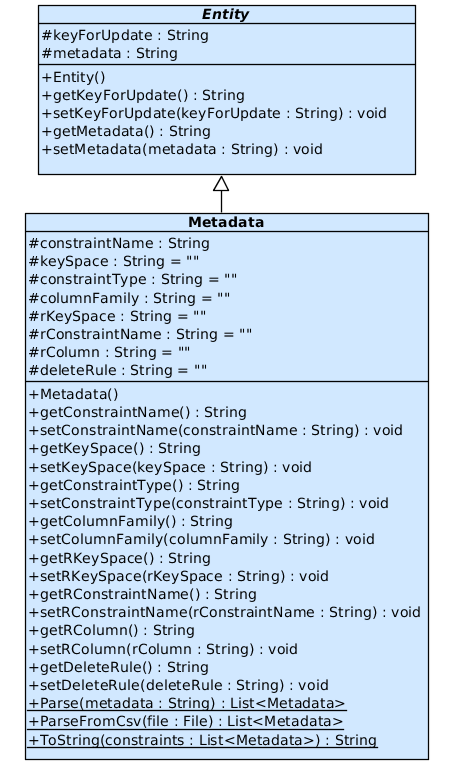
\includegraphics[width=.5\textwidth]{./figure/uml/metadata.png}
		\caption{Metadata Entity Class}\label{fi:MetadataEntityClass}
	\end{figure}
	
The \texttt{ValidationHandler} retrieves the list of \texttt{Metadata} entities
relevant to the entity upon validation.  In this case, it does so by using the
\texttt{EntityManager} to read the constraints from \texttt{Metadata}.  The
\texttt{Validation\-Handler} iterates through the list of 
\texttt{Metadata} entities and uses the respective getter methods in order to
retrieve the different attributes of the metadata to complete the validation. 
Notice that, in Solution~4, the list of metadata is maintained in
cache in order to re-use it for future validations and to avoid additional 
connections to the metadata cluster each time validation needs to be 
performed.


\subsection{Metadata as Text}\label{ss:implementation-MDText}

Solutions~1 and 2 store metadata as a string of text. Solution~1 stores the
metadata within each entity in its  \texttt{Metadata} column, and
 Solution~2 stores the metadata in  the top row of the respective column
families. Notice that, Solution~2 performs an additional
 search to locate the  top row (\texttt{RowId=`-1'}) where the metadata is
 stored, and then loads it within the  entity.
 
The string of metadata within each entity contains all the constraints
 separated using special characters as explained in Section~\ref{s:design-sol1}.
These special characters serve as delimiters to
parse and extract the information about the relevant constraints. This
 information is then loaded into the attributes of an instance of the
\texttt{Metadata} entity class and, from then on, metadata is handled as an
 entity as explained in the previous section.  Notice that the parsing
algorithms for metadata as string are provided as static members of
\texttt{Metadata} class.
 
%   Basically, the
%  \texttt{ValidationHandler} uses the relevant getter methods of the
%  \texttt{Metadata} entity class to retrieve  the different attributes necessary
% to complete the validation.






% Each time an entity is loaded, the
% \texttt{EntityManager} parses its string of metadata using the special
% characters as delimiters, in order to extract each constraint and its associated
% values. 











